\documentclass[12pt]{article}
\usepackage[utf8]{inputenc}
%\usepackage{csquotes}
\usepackage{graphicx}
\graphicspath{ {pictures/} }
\usepackage{caption}
\usepackage{subcaption}
\usepackage[a4paper,width=150mm,top=25mm,bottom=25mm,bindingoffset=6mm]{geometry}
\usepackage[english, ngerman]{babel}
\usepackage{amsthm,etoolbox, amsmath, amssymb}
\usepackage{enumitem}   
\usepackage[nottoc]{tocbibind}
\usepackage{hyperref}
\usepackage{wrapfig}
\usepackage{color} 
\usepackage{algorithm}
\usepackage{algpseudocodex}
\usepackage{aligned-overset}
\usepackage [autostyle, german = quotes]{csquotes}
\usepackage{tikz}
\usepackage{pgffor}
\usepackage{listings}
\usepackage{fancyhdr}
\MakeOuterQuote{"}

\AddToHook{cmd/section/before}{\clearpage}

\theoremstyle{plain}
\newtheorem{thm}{Theorem}
\newtheorem{lem}[thm]{Lemma}
\newtheorem{prop}[thm]{Proposition}
\newtheorem{cor}[thm]{Korollar}

\theoremstyle{definition}
\newtheorem{definition}[thm]{Definition}
\newtheorem{ex}[thm]{Beispiel}

\theoremstyle{remark}
\newtheorem{rem}[thm]{Bemerkung}

\makeatletter
\@addtoreset{thm}{section}% Reset theorem counter with every section
\@addtoreset{thm}{subsection}
\@addtoreset{thm}{subsubsection}
\newcommand{\theoremprefix}{}
\let\thetheoremsaved\thethm
\renewcommand{\thethm}{\theoremprefix\thetheoremsaved}
\let\sectionsaved\section
\patchcmd{\@startsection}{\par}{\renewcommand{\theoremprefix}{\csname the#1\endcsname.}}{}{}
\makeatother

\setlength{\jot}{10pt}
\setlength{\headheight}{15pt}

\newcommand*\circled[1]{\tikz[baseline=(char.base)]{%
            \node[shape=circle,fill=blue!20,draw,inner sep=2pt] (char) {#1};}}

\usepackage[style=alphabetic, firstinits=true, backend=biber, sorting=nyt, doi=false, isbn=false, url=true, maxbibnames=99]{biblatex}
\DeclareNameAlias{default}{family-given}
\addbibresource{references.bib}

\title{Thesis Title}
\author{Author Name}
\date{Day Month Year}

\setlength\parindent{0pt}

\begin{document}
	\begin{titlepage}
	\begin{center}
		\vspace*{1cm}
		\includegraphics[scale=0.1]{KTH_Royal_Institute_of_Technology_logo.svg.png}\\
		\Large
		KTH Stockholm\\
		Department of Numerical Analysis
		\vspace*{1cm}



		\Huge
		\textbf{Towards generating privacy-preserving and useful time series ECG data for arrhythmia detection
		}
		
		\vspace{0.5cm}
		
		\vspace{1.5cm}
		
		
		\vfill
		
		Master Thesis Report \\
		Sijun John Tu
		\vspace{0.8cm}

		
		\large
		Supervisors: Anders Szepessy (KTH) and Shahid Raza (RISE)\\
		
	\end{center}
\end{titlepage}
	
\subsubsection*{Abstract}

    In this paper, we investigate the so-called numerical value range of a linear, bounded operator in a Hilbert space. Similar to the spectrum of an operator, the numerical range of values helps to determine certain properties of the corresponding operator to be investigated. In doing so, we will often encounter relations between there two invariants. The main objective of this section is the so-called Power Inequality, a statement about the numerical radius of powers of an operator, as well as the norm property of the numerical radius. In particular, an algorithm is presented and implemented, which numerically approximates the numerical value for a finite-dimensional operator. In the final chapter of the thesis, an application of the numerical value range in numerical mathematics is considered.


	\thispagestyle{empty}
\section*{Eidesstattliche Erklärung}

Hiermit erkläre ich, dass ich die vorliegende Arbeit selbstständig und eigenhändig sowie ohne unerlaubte fremde Hilfe und ausschließlich unter Verwendung der aufgeführten Quellen und Hilfsmittel angefertigt habe.\\

Die selbstständige und eigenhändige Anfertigung versichert an Eides statt:\\\\\\\\\\
Berlin, den \today \\[5cm]
\rule{10cm}{0.4pt}\\
Sijun John Tu
	\tableofcontents
	\thispagestyle{empty}
	% \addtocontents{toc}{\protect\thispagestyle{empty}}
	\setcounter{page}{0}

	
\section*{Notation}
Mathematical conventions and notation used in this thesis:

\begin{center}
    \renewcommand{\arraystretch}{1.5}
    \begin{tabular}{ c l }
        
        $\mathbb{R}$ & the real numbers \\
        $\sqcup$ & disjoint set union \\
        $\mathcal{N}(\mu, \sigma^2)$ & Gaussian distribution with mean $\mu$ and variance $\sigma^2$
    \end{tabular}
\end{center}

Additionally, we introduce the following conventions to describe various elements from different mathematical objects to make the notations and their meaning as consistent as possible:

\begin{center}
    \renewcommand{\arraystretch}{1.5}
    \begin{tabular}{c l}
        $\mathcal{S}$ & set of heartbeat samples \\
        $s_i \in \mathbb{R}^L$ & seqeunce of ECG measurements \\
        $\mathcal{K}^X$ & arrhythmia detection model trained on some training data $X$


    \end{tabular}
\end{center}

	\addcontentsline{toc}{section}{Notation}

	\listoffigures

	\pagestyle{fancy}
	\fancyhf{}
	\fancyhead[L]{\leftmark}
	\fancyfoot[R]{\thepage}


	\section{Mathematische Grundlagen}
	\begin{frame}
    % Print the title page as the first slide
    \titlepage
\end{frame}

\begin{frame}{Outline}
    % Throughout your presentation, if you choose to use \section{} and \subsection{} commands, these will automatically be printed on this slide as an overview of your presentation
    \tableofcontents
\end{frame}
	
	\section[Numerischer Wertebereich und numerischer Radius]{Numerischer Wertebereich und \\numerischer Radius}
	\section{Project introduction}

\begin{frame}
    \frametitle{Machine Learning Pipeline}
    \tikz{
            \node[circle,fill=Button1,inner sep=3pt] (c) at (0,0){};
            \node[circle,fill=Button2,inner sep=3pt] (c) at (0.5,0){};
            \node[circle,fill=Button3,inner sep=3pt] (c) at (1,0){};
        }~~~~~~\textcolor{gold}{Figure: }High-level machine learning pipeline
    \begin{figure}[h]
        
        \centering
        \includegraphics[scale=0.45]{ml_pipeline.png}
    \end{figure}
\end{frame}



\begin{frame}{Anomaly detection using privacy-preserving, synthetic time series data}
    
    \begin{itemize}
        \item<1-> Problem
        \begin{itemize}
            \item<1-> ML models are very \alert{data hungry}.
            \item<1-> In many cases sharing data comes with \alert{privacy risks}.
        \end{itemize}
        \item<2-> Solution:
        \begin{itemize}
            \item<2-> Promising solution: \alert{synthetic data} with privacy guarantees!
            \item<2-> Synthetic data with \alert{differential private} (DP) guarantees is a promising solution to ensure privacy independent of downstream task.
        \end{itemize}
        \item<3-> BUT:
        \begin{itemize}
            \item<3-> \alert{Privacy-Utility-Tradeoff}: Commonly, a gain in privacy results in a loss of utility. 
            \item<3-> For \alert{anomaly detection} this might not be the case (?).
        \end{itemize}
    \end{itemize}
\end{frame}


\begin{frame}{Structure}
    
    \begin{figure}[h]
        \begin{flushleft}
            \tikz{
            \node[circle,inner sep=3pt] (c) at (-0.5,0){};
            \node[circle,fill=Button1,inner sep=3pt] (c) at (1.0,0){};
            \node[circle,fill=Button2,inner sep=3pt] (c) at (1.5,0){};
            \node[circle,fill=Button3,inner sep=3pt] (c) at (2.0,0){};
        }~~~~~~\textcolor{gold}{Figure: }Structure of Experiment pipeline
        \end{flushleft}
        \centering
        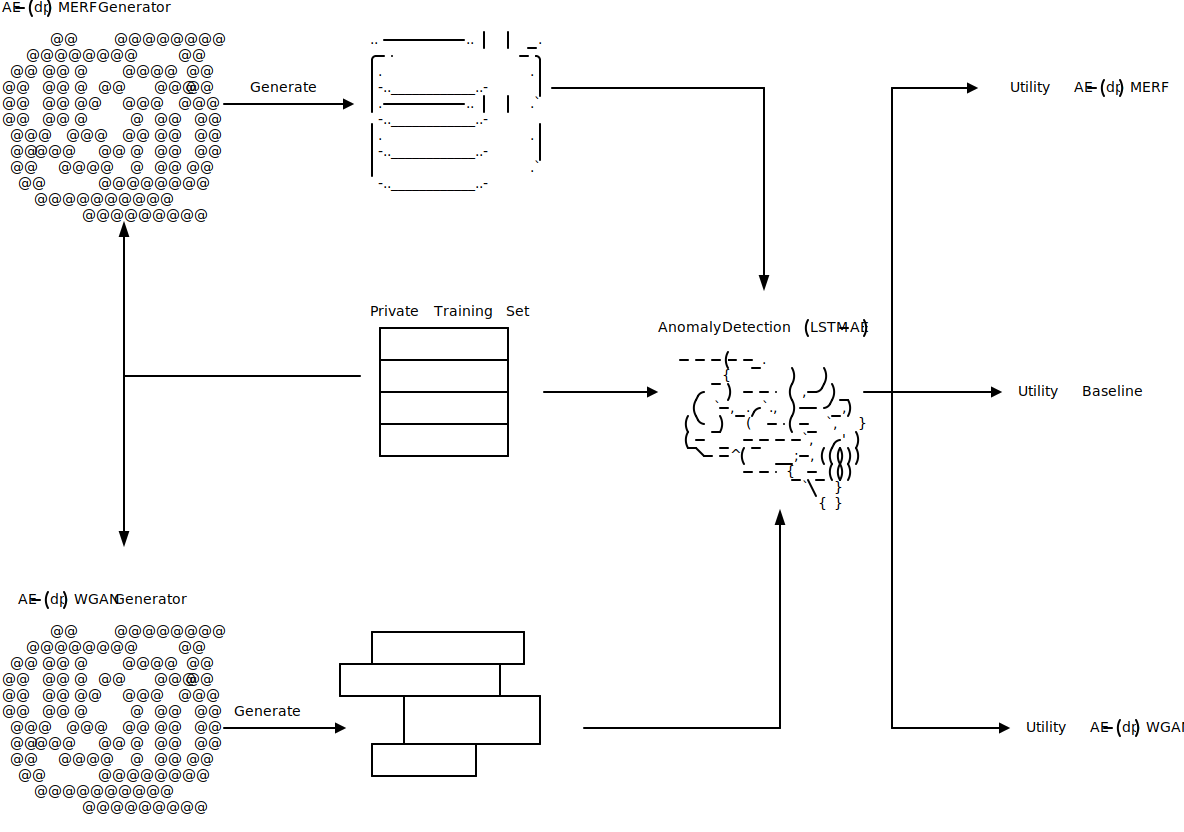
\includegraphics[scale=0.28]{str.png}
    \end{figure}
\end{frame}

\begin{frame}{Structure}
    \begin{enumerate}
        \item<1-> Train \alert{baseline model} for anomaly detection only on \alert{regular, private heartbeat data} using an LSTM-Autoencoder.
        \item<2->  \alert{Generate regular heartbeat} data using two approaches:
        \begin{itemize}
            \item<2-> [--] AE-(dp)MERF
            \item<2-> [--] AE-(dp)WGAN
        \end{itemize}
        \item<3->  Train LSTM-Autoencoder for \alert{anomaly detection on synthetic data} and \alert{test on real}.
        \item<3-> Assess \alert{utility} by measuring performance for anomaly detection (Accuracy, precision, recall, F1). 
        \item<4->  \alert{Contaminate} training data with anomalous heartbeats and repeat.
    \end{enumerate}
\end{frame}




	\section[Lax-Wendroff-Verfahren ]{Lax-Wendroff-Verfahren}
	\section{Dataset: MITBIH ECG data}
\begin{frame}{Heartbeat Arrhythmia}
    \begin{figure}
        \centering
        \includegraphics[scale=0.3]{images/heartbeat_arr.png}
        \caption[]{Different heartbeat arrhythmias \footnote{source: https://www.parkwayshenton.com.sg/health-plus/article/arrhythmia-guide}}
        \label{fig:enter-label}
    \end{figure}
\end{frame}

\begin{frame}{Arrhythmia Detection as an Anomaly Detection Problem}
We treat the problem of detecting anomalous heartbeats as an anomaly detection problem from machine learning based on the \alert{reconstruction error}:
\begin{itemize}
    \item<2->  We train a model \alert{on regular heartbeats} that is able to reconstruct that regular heartbeat.
    \item<3->  Given an anomalous heartbeat the model should give \alert{higher reconstruction error}.
    \item<4->  Based on an optimal \alert{threshold} for that error we classify this heartbeat as either regular or anomalous.
\end{itemize}
    \onslide<5>{Two reasons for this semi-supervised approach: high class imbalancy and no need for labelling.}
\end{frame} 

\begin{frame}{Baseline Model}
    Model is a LSTM-AE that is \alert{trained only on regular, private samples} with the goal to reconstruct normal samples. The classification is made based on the reconstruction error.
    \begin{columns}
        \begin{column}{0.48\textwidth}
        \begin{figure}
            \centering
            \includegraphics[scale=0.3]{images/rec_normal.png}
            \caption{reconstruction on normal sample \phantom{asdfsadf}}
            \label{fig:enter-label}
        \end{figure}
    \end{column}
    \begin{column}{0.48\textwidth}
        \begin{figure}
            \centering
            \includegraphics[scale=0.3]{images/rec_anom.png}
            \caption{reconstruction on anomalous sample}
            \label{fig:enter-label}
        \end{figure}
    \end{column}
    \end{columns}
\end{frame}



	\clearpage

	\fancyhead[L]{ANHANG}
	\section*{Anhang}
	\addcontentsline{toc}{section}{Anhang}
	\section*{Appendix}

In \cref{chapter5} we omitted some plots in regards to the data generation process which we attach here.

\subsection*{Training anomaly detection on AE-dpMERF data}

\subsubsection*{Using $\epsilon=1$}

\begin{figure}[H]
    \centering
    \includegraphics[scale=0.7]{loss_aedpmerf_eps1.png}
    \caption{Loss over epoch for anomaly detection model trained on AE-dpMERF generated data with $\epsilon=1$ together with loss on validation set}
\end{figure}

\begin{figure}[h]
    \begin{minipage}[b]{0.45\textwidth}
        \centering
        \includegraphics[scale=0.4]{hist_threshold_aedpmerf_eps1.png}
        \caption{Distribution of reconstruction error on validation set with AE-dpMERF with $\epsilon=1$ generated samples}
    
    \end{minipage}
    \begin{minipage}[b]{0.45\textwidth}
        \centering
        \includegraphics[scale=0.4]{thres_plot_aedpmerf_eps1.png}
        \caption{Percentage of correctly classified regular and anomalous test samples for different threshold values with AE-dpMERF with $\epsilon=1$ generated sampled}
        \label{fig:thres_aegwan}
    \end{minipage}
\end{figure}

\subsubsection*{Using $\epsilon=0.5$}

\begin{figure}[H]
    \centering
    \includegraphics[scale=0.7]{loss_aedpmerf_eps05.png}
    \caption{Loss over epoch for anomaly detection model trained on AE-dpMERF generated data with $\epsilon=0.5$ together with loss on validation set}
\end{figure}

\begin{figure}[h]
    \begin{minipage}[b]{0.45\textwidth}
        \centering
        \includegraphics[scale=0.4]{hist_threshold_aedpmerf_eps05.png}
        \caption{Distribution of reconstruction error on validation set with AE-dpMERF with $\epsilon=0.5$ generated samples}
    
    \end{minipage}
    \begin{minipage}[b]{0.45\textwidth}
        \centering
        \includegraphics[scale=0.4]{thres_plot_aedpmerf_eps05.png}
        \caption{Percentage of correctly classified regular and anomalous test samples for different threshold values with AE-dpMERF with $\epsilon=0.5$ generated sampled}
        \label{fig:thres_aegwan}
    \end{minipage}
\end{figure}

\subsubsection*{Using $\epsilon=0.1$}

\begin{figure}[H]
    \centering
    \includegraphics[scale=0.7]{loss_aedpmerf_eps01.png}
    \caption{Loss over epoch for anomaly detection model trained on AE-dpMERF generated data with $\epsilon=0.1$ together with loss on validation set}
\end{figure}

\begin{figure}[h]
    \begin{minipage}[b]{0.45\textwidth}
        \centering
        \includegraphics[scale=0.4]{hist_threshold_aedpmerf_eps01.png}
        \caption{Distribution of reconstruction error on validation set with AE-dpMERF with $\epsilon=0.1$ generated samples}
    
    \end{minipage}
    \begin{minipage}[b]{0.45\textwidth}
        \centering
        \includegraphics[scale=0.4]{thres_plot_aedpmerf_eps01.png}
        \caption{Percentage of correctly classified regular and anomalous test samples for different threshold values with AE-dpMERF with $\epsilon=0.1$ generated sampled}
        \label{fig:thres_aegwan}
    \end{minipage}
\end{figure}

\subsubsection*{Using $\epsilon=0.01$}

\begin{figure}[H]
    \centering
    \includegraphics[scale=0.7]{loss_aedpmerf_eps001.png}
    \caption{Loss over epoch for anomaly detection model trained on AE-dpMERF generated data with $\epsilon=0.01$ together with loss on validation set}
\end{figure}

\begin{figure}[H]
    \begin{minipage}[b]{\textwidth}
        \centering
        \includegraphics[scale=0.4]{hist_threshold_aedpmerf_eps001.png}
        \caption{Distribution of reconstruction error on validation set with AE-dpMERF with $\epsilon=0.01$ generated samples}
    
    \end{minipage}
    \begin{minipage}[b]{\textwidth}
        \centering
        \includegraphics[scale=0.4]{thres_plot_aedpmerf_eps001.png}
        \caption{Percentage of correctly classified regular and anomalous test samples for different threshold values with AE-dpMERF with $\epsilon=0.01$ generated sampled}
        \label{fig:thres_aegwan}
    \end{minipage}
\end{figure}




\subsection*{Training anomaly detection on AE-dpWGAN data}

\subsubsection*{Using $\epsilon=35$}


\begin{figure}[H]
    \begin{minipage}[b]{\textwidth}
        \centering
        \includegraphics[scale=0.4]{hist_threshold_aedpwan_eps35.png}
        \caption{Distribution of reconstruction error on validation set with AE-dpWGAN with $\epsilon=35$ generated samples}
    
    \end{minipage}
    \begin{minipage}[b]{\textwidth}
        \centering
        \includegraphics[scale=0.4]{thres_plot_aedpwgan_eps35.png}
        \caption{Percentage of correctly classified regular and anomalous test samples for different threshold values with AE-dpWGAN with $\epsilon=35$ generated sampled}
        \label{fig:thres_aegwan}
    \end{minipage}
\end{figure}

\subsubsection*{Using $\epsilon=25$}

\begin{figure}[H]
    \begin{minipage}[b]{\textwidth}
        \centering
        \includegraphics[scale=0.4]{hist_threshold_aedpwgan_eps25.png}
        \caption{Distribution of reconstruction error on validation set with AE-dpWGAN with $\epsilon=25$ generated samples}
    
    \end{minipage}
    \begin{minipage}[b]{\textwidth}
        \centering
        \includegraphics[scale=0.4]{thres_plot_aedpwgan_eps25.png}
        \caption{Percentage of correctly classified regular and anomalous test samples for different threshold values with AE-dpWGAN with $\epsilon=25$ generated sampled}
        \label{fig:thres_aegwan}
    \end{minipage}
\end{figure}

\subsubsection*{Using $\epsilon=5$}


\begin{figure}[H]
        \centering
        \includegraphics[scale=0.4]{hist_threshold_aedpwgan_eps5.png}
        \caption{Distribution of reconstruction error on validation set with AE-dpWGAN with $\epsilon=5$ generated samples}
\end{figure}

\begin{figure}[H]
        \centering
        \includegraphics[scale=0.4]{thres_plot_aedpwgan_eps5.png}
        \caption{Percentage of correctly classified regular and anomalous test samples for different threshold values with AE-dpWGAN with $\epsilon=5$ generated sampled}
        \label{fig:thres_aegwan}
\end{figure}
	\clearpage

	\pagestyle{fancy}
	\fancyhead[L]{LITERATURVERZEICHNIS}
	\fancyfoot[R]{\thepage}
	\printbibliography[heading=bibintoc, title=Literaturverzeichnis]
\end{document}
